%%% THIS IS THE TEMPLATE, MODIFIED FROM THE COMPUTER SCIENCE
%%% TEMPLATE OF THE UNIVERSITY OF HELSINKI
\documentclass[officiallayout]{tktla_modified}
%\documentclass[officiallayout,a4frame]{tktla}

%%%% ALL THE PACKAGES TO BE USED FOR THE DOCUMENT
\usepackage[latin1]{inputenc}
\usepackage{latexsym}
\usepackage{graphicx}
\usepackage{nomencl}
\renewcommand{\nomname}{Abbreviations}
\usepackage[round]{natbib}
%\bibliographystyle{plainnat}
\bibliographystyle{chicago}
%\usepackage[nottoc]{tocbibind}
\usepackage[T1]{fontenc}

%%%

\usepackage[framemethod=TikZ]{mdframed}
\usepackage{fancyref}
\mdfdefinestyle{boxstyle}{%
rightline=true,
innerleftmargin=10,
innerrightmargin=10,
frametitlerule=true,
frametitlerulecolor=red!15,
backgroundcolor=red!15,
frametitlerulewidth=2pt}

\renewcommand{\theenumi}{\roman{enumi}}


%%%%%%%%%%%%%%%%%%%%%%%%%%%%%%%%%%%%%%%%%%%%%%%%%%%%%%%%%%%%%%%%%%%%%%%%%%%
%% ------Data to produce the front page ------------
\title{Estimating complexity and adaptation in space and time in the embryo
%:\\ A statistical developmental biology approach
}
\author{Irepan Salvador-Mart\'inez}
\authorcontact{irepan.salvador@helsinki.fi\par
  http://cs.helsinki.fi/John.Smith/}
\pubtime{November}{2016}
\reportno{0}
\isbnpaperback{000-00-0000-0}
\isbnpdf{000-00-0000-0}
\issn{1238-8645}
\printhouse{Unigrafia}
\pubpages{7} % --- remember to update this! 

% For article-based theses, the number of the last page of the list of
% references of the preamble part + the total number of the pages of
% the original articles and interleaf pages.

%% ------Data to produce the Supervisor/Custos ------------
\supervisorlist{Isaac Salazar-Ciudad, University of Helsinki, Finland}
\preexaminera{Pavel Tomancak, Max Planck Institute of Molecular Cell Biology and \par
              \quad\quad Genetics in Dresden, Germany}
\preexaminerb{Gregor Bucher, Georg-August-University G{\"o}ttingen, Germany}
\opponent{Johannes J{\"a}ger, Konrad Lorenz Institute, Austria}
\custos{Name, University, Country}
%\generalterms{thesis, example, another example, still more examples,
%  more and more examples}
%\additionalkeywords{example, an example phrase with many words}
%\crcshort{A.0, C.0.0}
%\crclong{
%\item[A.0] Example Category
%\item[C.0.0] Another Example
%}
\permissionnotice{
  To be presented in \ldots{} text of a long permission notice. Text of
  a long permission notice. Text of a long permission notice. Text of
  a long permission notice. Text of a long permission notice. Text of
  a long permission notice.
}

%\newtheorem{theorem}{Theorem}[chapter]
%\newenvironment{proof}{\noindent\textbf{Proof.} }{$\Box$}

%%%%%%%%%%%%%%%%%%%%%%%%%%%%%%%%%%%%%%%%%%%%%%%%%%%%%%%%%%%%%%%%%%%%%%%%%%%
%%%% -----------------------------------------------------------------
%%%% ----------------BEGIN OF THE DOCUMENT----------------------------

\begin{document}

\frontmatter

\maketitle
\makenomenclature
%\begin{abstract}
%\end{abstract}

\begin{acknowledgements}
  
\end{acknowledgements}


\tableofcontents

\mainmatter

%%%% -----------------------------------------------------------------
%%%% ---------- BEGIN OF THE MAIN TEXT -------------------------------
%%%% -----------------------------------------------------------------
%%%% -----------------------------------------------------------------

\mychapter{0}{List of publications}


%%%% -----------------------------------------------------------------
%%%% ---------ABREVIATIONS------------------------------------------

\printnomenclature

%%%% -----------------------------------------------------------------
%%%% ---------- ABSTRACT---------------------------------------------

\chapter{Abstract}
	
Embryonic development has amazed scientists and philosophers for centuries.

Many reasons have been evoked for the perceivable complexity increase that transforms a single cell into a larva or an adult (even when complexity has eluded an unique definition).
Aristotle claimed a "vital force" guided embryogenesis. %Eventually, 
Vitalism was substituted by preformationism and epigenesis explanations in the 18th century.
%
Since the 1980's, when it became clear that genes play a key role in embryogenesis, 
%Nowadays, 
the causal mechanisms for such complexity increase are being searched for at the cellular and molecular level.

Using the number of cell types as complexity measure, its increase during development is self-evident: the embryo begins with one cell type (zygote) and concludes with up to 200 cell types (in mammals). 
This process can also be called embryo compartmentalization.
%From many discoveries since the 1980's, it has become clear that some genes play a key role in the embryo compartmentalization. 
At the level of gene expression, it its assumed that in early development, genes are initially expressed in large domains on the embryo. Then, at later stages, their expression become spatially restricted, until some genes are expressed in a cell-specific manner.
%
For many crucial developmental genes (e.g., Hox genes), the spatio-temporal expression dynamics, and how it relates to the embryo compartmentalization, has been thoroughly described.
It is not clear however, if the dynamics are similar for the rest of the genes deployed in development, or if there are differences between different types of genes.

-----------------------------

Adaptive reasons have been also said to be the cause for the increase in complexity.
A change during development would be adaptive if it increases the fitness of its bearer, even when the effect of this developmental change is realized until the adult or larva.
%The increase in complexity (or any change in development) has been considered for some authors as the adaptations of the embryo to its environment.

Many methods of molecular evolution estimate the action of natural selection based on the quasi-neutral evolution model.
Under this model, an adaptive change that has been caused by a genetic mutation, can be traced in the DNA sequence, as a positive selected site would show less variance than other sites evolving neutrally.

Recently, methods of population genomics use divergence ans polymorphism (inter-specific and intra-specific variation) to measure more precisely the proportion of adaptive mutation at the molecular level.

----------------------------
Importantly, if different developmental stages show distinct levels of positive selection or stabilizing selection,
some specific patterns, when comparing the development trajectories of different species in a group, might be recognizable.
% specific patterns might appear (patterns of what?) when comparing the divergence between different species.
Two related models currently under much discussion? are:
%This is related to already proposed models of divergence: 
1)von Baer's laws and the hourglass model.
The former states that the development of 2 species would be very similar in early stages and increasingly divergent in subsequent stages. In contrast, the latter states that development is less divergent at mid development.

%Such patterns could be due to selection or constrant..
%The print in natural selection on the genome is useful to discern between these scenarios.
%Some regarded each embryonic stage to have adaptation as the result of the constant interaction of the embryo with its environment (whether external or internal).
%Others have distinguished the adaptations in the embryo from those from the adult, stating that the former are product of internal selection, instead of being product of natural selection, as the latter.
------------------------------------------
In here, I will use gene expression information to estimate 
both complexity and adaptation in the embryo.

I will use a statistical approach, this means that no special emphasis on specific genes or pathways would be made. 
Instead, my intention is to provide a broad picture on the spatiotemporal change in complexity and adaptation in the embryo.

%I take advantage of available databases of gene expression.
%I analyze complexity using two popular developmental biology models: Drosophila melanogaster and Ciona intestinalis.
For the estimation of complexity, I analyzed gene expression data (from thousands of in situ hybridization experiments) of two popular developmental biology models: Drosophila melanogaster and Ciona intestinalis (from available databases) and developed quantitative measures of complexity.

To analyze adaptation, I combined the D. melanogaster transcriptomic data with genomic data from the DGRP project. With the DFE-alpha method (which uses coding-region polymorphism data and coding-region divergence between D. yakuba and D. melanogaster to estimate the proportion of adaptive changes), I chart a spatial map of adaptation of the fruit fly embryo's anatomy. 

Also, I analyze the pattern of positive selection through the entire life cycle of D. melanogaster.

Briefly, 

we found that low rates of adaptive change are found in the digestive system and high rates in the gonads and parts of the forming head. We also found that the regions that exhibit the highest rates of adaptation express, on average, genes that are phylogenetically young

%%%% -----------------------------------------------------------------
%%%% -----------------------------------------------------------------

\chapter{Review of the literature}
	
An example for citation is here 
\citep{Tomancak2002}.
Bibliography automatically build at the end. Also an example of abbreviation with the BDGP database
	\nomenclature{DGRP}{Drosophila Genome Reference Panel}	
	\nomenclature{BDGP}{Berkeley Drosophila Genome Project}
and DGRP
is just here.
	

	\section{Complexity}
	
The increase in complexity in an organism during embryogenesis is probably one of the most intuitive processes of animal development, 
even when there is no consensus definition of what exactly complexity is and how complexity should be measured.


A general definition could be "the number of component parts" of an organism.
These "parts" might be body segments (e.g., of an insect) or genes
	\citep{Arthur2010}.
It is evident that these definitions are problematic.
It is doubtful to say that some centipede is more complex than a beetle, just based in the different number of segments they have.
Also, it is already acknowledge that there is no relation between the number of coding-genes and morphological complexity.
This lack of correspondence, sometimes referred as the "G-value paradox"
	\citep{Hahn2002},
became evident with the release of the first eukaryotic genome sequences.
Decades before, the lack of correspondence between genome size and organism complexity (or "C-value paradox") was also noted.


An alternative definition of complexity includes not only the "number of parts" but also the "interaction among parts" 
	\citep{Arthur2010}.
This could be illustrated with the number of gene-gene interactions (e.g., expression regulation by a transcription factor binding to a promoter region of another gene),
such that when comparing two different organisms that have same number of genes, 
one organism could be considered to be more complex than the other if the former has more gene-gene interactions than the latter.
Again this definition is disputable, as it is acknowledged that during evolution gene-gene interactions (or gene regulatory network) underlying a phenotype
can increase their complexity without affecting the phenotype itself
	\citep{Muller1999,True2001,Salazar-Ciudad2009}.

\subsection{Complexity Increase in Evolution and Development}

The increase in complexity in evolution has has been a topic of interest for more than a century.
Early views of evolution saw the increase in complexity as inexorable, with all the species descending
from simpler ancestral forms and with the human species as the latest and more perfect product of 
the evolution of animals
	(REF Haeckel).
Recent views recognize that within a phylum complexity of the species can increase or decrease.

-parasites

-cave animals

-it is the range od complexity that increases


connection with development


	
\subsection{Complexity as number of cells}

A measure of morphological complexity that has been favoured by some authors (perhaps because of its intuitiveness), is the number of cell types that compose an organism 
	\citep{Bell1997,Bonner2004,McShea1996}.
Using the number of cell types as a proxy of morphological complexity, it can be said that during metazoan development, complexity increases as the zygote divides and differentiates into an adult with multiple cell types. This simple definition of complexity has its complications, as there are no clear-cut consensus criteria about how to define a cell type or about when a new cell type has arisen during development. 
However, even using this simple definition of complexity has its complications, as there is no clear criteria of how to define a cell type or how to determine when a new cell type has formed during development. It could be that at the morphological level a cell seems to be undifferentiated, but when isolating it, it differentiates in an autonomous way into a specific cell type, suggesting that the cell fate was already determined without the necessity of further interactions with other cells. 
In addition, this definition does not take into account that embryos do not only get more cell types, they also organize them in specific patterns in space that seem to increase in complexity over developmental time.

	
\subsection{Complexity at the molecular level}


At the level of gene expression it seems also clear that the embryo becomes progressively compartmentalized over time and space. In spite of this intuitiveness, there

	\clearpage 
	\section{Adaptation}
	Measuring adaptation is an important topic in evolutionary biology.

Since Darwin.. (REF Darwin)

In here, I refer to adaptation as a phenotypic character (or modification in a phenotypic character) that arise by natural selection in response to the environment, or other external factor.
Measuring adaptation at the phenotypic level requires a clear understanding of the function of the phenotypic character under study, and how the modification of this trait would affect the fitness of the bearer organism 
	\citep{EmiliaSantos2015}. 

Importantly, all phenotypic changes (whether a new character or a modification of an existing character) is produced from a change in development.
For example, the difference in the beak size and shape between the famous Galapagos Darwin's finches (REF Darwin), a classic example of adaptive change under natural selection, has been shown to be regulated by the differential expression of the genes CaM 
	\nomenclature{CaM}{Calmoduline}
and BMP4 
	\nomenclature{BMP4}{Bone morphogenetic protein 4}
during development. A proposed model for BMP4 and CaM role in beak size and shape explains both elongated and deep/wide beaks of these finches
	\citep{Abzhanov2006}.

So, even when natural selection acts in the adult phenotype (or in the larva, in the case of species with a feeding larva stage), we should be able to find changes in development that would explain an adaptive change in the adult or larva.


Some other remarkable examples of the genetic-developmental basis of adaptive change are:

-

-

It is evident at this point than many of the developmental changes leading to an adaptation are (at least partially) caused by mutations in gene regulatory or coding sequences.
Therefore, the effects of natural selection could be traceable looking at the adaptive changes in the genes expressed in different times and locations during development. There is an entire field within evolutionary biology, namely molecular evolution, dedicated to explain the sequence changes in molecules as DNA,
	\nomenclature{DNA}{Deoxyribonucleic acid}
RNA 
	\nomenclature{RNA}{Ribonucleic acid}
and proteins. 


\subsection{Molecular evolution}

The theoretical basis of the molecular evolution field includes concepts from evolutionary biology and population genetics. At the DNA level, any transmissible change in the sequence is considered a mutation. 
The most simple change is a point mutation or single nucleotide polymorphism (SNP),
\nomenclature{SNP}{Single nucleotide polymorphism} 
which is a change in a single nucleotide in the DNA sequence of a locus of two individuals. 
If the individuals belong to the same species, this mutation is referred as polymorphism. In contrast, divergence refers to the mutations when individuals from different species are taken into account. 
SNPs occur in non-coding and coding DNA sequence. A single point mutation that occurs in a coding sequence can be classified in two categories, depending on the effect of this mutation in the protein sequence: i) synonymous mutation and ii) non-synonymous mutation.
A synonymous mutation does not affect the amino-acid sequence of the protein, albeit it can affect its function 
	\citep{Kimchi-Sarfaty2007}
or the gene transcriptional efficiency (REF).
A non-synonymous mutation does affect the amino-acid sequence of the protein whether by changing a single amino-acid (missense mutation) or by producing a stop codon (non-sense mutation) which results in a truncated version of the protein.

As the non-synonymous mutations can affect dramatically the structure and function of the protein, it is expected that most of non-synonymous mutations would have a negative fitness effect.
However, it is also expected that a fraction of non-synonymous mutations, or adaptive substitutions, would have a positive fitness effect that (depending on the strength of the fitness effect) could lead to the fixation of that mutation in the population.

An important branch of the molecular evolution field is dedicated to the identification of adaptive substitutions in a species, which has lead to the development of many statistical tests. 
Importantly, these tests are based on the neutral theory of evolution, proposed by Kimura
	\citep{Kimura1968}.

\subsection{Neutral theory of evolution}
In 1968, Mooto Kimura calculated the average rate of nucleotide substitutions in the evolutionary history of mammals.
The result of his calculations was that, on average, one nucleotide has been substituted every 2 years.
For him, this very high rate of substitution was only explainable if most mutations were almost neutral in natural selection 
	\citep{Kimura1968}.
This was in contrast with the prevailing view at the time that practically no mutations are neutral (REF).
More importantly, the neutral theory provided a set of testable predictions, providing a null-hypothesis of molecular evolution.
This allowed the development of statistical methods to detect adaptive changes, i.e., we can say that a sequence has been under positive selection if the amount of changes exceeds the number of changes expected only by neutral evolution.
One of the most popular tests is the McDonald-Kreitman test (MKT),
	\nomenclature{MKT}{MacDonald-Kreitman test}
which estimates the proportion of the adaptive substitution resulted from natural selection.

\subsection{McDonald-Kreitman test}
John H. McDonald and Martin Kreitman developed this test in 1991 when analysing the divergence in the Adh 
	\nomenclature{Adh}{Alcohol dehydrogenase}
locus in three Drosophila species
	\citep{McDonald1991}.
The main assumption of the MKT is that the substitutions in a protein are neutral if the 
inter-specific ratio of non-synonymous (Dn) to synonymous (Ds) changes is equal to the 
intra-specific ratio of non-synonymous (Pn) to synonymous (Ps) changes (i.e. Dn/Ds = Pn/Ps).
Any departure from these equality would imply the action of positive or negative selection.
If some of the changes are result from positive selection, the ratio of non-synonymous to synonymous variation within species should be lower than the ratio of non-synonymous to synonymous variation between species (i.e. Dn/Ds > Pn/Ps). 
In the case that the observed ratio of non-synonymous to synonymous variation between species is lower than the ratio of non-synonymous to synonymous variation within species (i.e. Dn/Ds < Pn/Ps) 
then negative selection is at work.

Since mutations under positive selection spread through a population rapidly, they don't contribute to polymorphism but do have an effect on divergence.

Although the MKT has been proved robust to many sources of error (e.g., variation to mutation rate across the genome), it can underestimate the proportion of adaptive changes in the presence of slightly deleterious mutations
	 \citep{Messer2013,Eyre-Walker2006a}.
Recently, more sophisticated methods based on the MKT have been developed to correct for underestimation of adaptive evolution in the presence of slightly deleterious mutations. 


\subsection{Distribution of Fitness Effects}

To have a more precise estimate of the proportion of adaptive substitutions it is important to consider the relative contributions of the different types of mutations, based on their fitness effects.
Because even when for simplicity the mutation effects are usually classified in advantageous, neutral, and deleterious, there is actually a continuum of selective effects, from strongly deleterious, 
to highly adaptive mutations	
	\citep{Eyre-Walker2007},
with weakly deleterious, neutral and slightly adaptive mutations in between.

The relative frequencies of all these type of mutations is called the Distribution of Fitness Effects (DFE).
	\nomenclature{DFE}{Distribution of Fitness Effects}
The DFE has other practical implications, like predicting the effects on the genetic variation in a population with low population size.
In order to know the DFE, a few experimental approaches exist. The most direct method is whether to induce 
	\citep{Sanjuan2004}
or to collect
	\citep{MUKAI1964}
spontaneous mutations and assay their effects (fitness) in the laboratory.
As can be expected, this experiments require many generations to gather sufficient data, so these approaches have been used mainly in micro organisms
	\citep{Eyre-Walker2007}.
A caveat of these experimental approaches is that, in order to identify the effect of a mutation, its effect has to be detectable in a fitness assay.
Therefore, these methods give valuable information for mutations with relatively large effects.

An alternative approach is to infer the DFE by analysing patterns of DNA sequence differences at intra and inter-specific level (polymorphism and divergence respectively).
The methods using this approach rely mainly on two assumptions:
i) the probability that a mutation spreads to a certain freq in a population (or to fixation) depends on the strength of selection (positive or negative) acting on it.
Severely deleterious mutations have lower probability to reach a high frequency in a population.
ii) the efficiency of selection depends on the effective population size. 
With a high effective population size, selection is more efficient and a smaller proportion of mutation will behave as effectively neutral.

The "absolute strength" of selection on a mutation is then measured as $N_{e}s$, the product of the effective population size ($N_{e}$)
	\nomenclature{$N_{e}$}{Effective population size}
by the selection coefficient ($s$)
	\nomenclature{$s$}{Selection coefficient}
of the mutation. Mutations with $N_{e}s$ much less than 1 are effectively neutral, while $N_{e}s$ greater than 100 have no chance to appear as polymorphism.

\subsection{DFE-alpha}

Eyre-Walker and collaborators 
	\citep{Eyre-Walker2009}
proposed a method to estimate both the DFE and the proportion of adaptive nucleotide substitutions ($\alpha$)
	\nomenclature{$\alpha$}{Proportion of adaptive nucleotide substitutions}
using polymorphism and divergence data.
More specifically, they use the polymorphism site frequency spectrum (SFS) 
	\nomenclature{SFS}{Site Frequency Spectrum}
to estimate the DFE and then use this estimated DFE to estimate the proportion of substitutions under positive selection between species.
This method, assumes that there are two types of nucleotide sites: 
i) sites at which all mutations are neutral and ii) sites at which some of the mutations are subject to selection (positive or negative).
Also it is assumed that any new adaptive mutation in a population would not be detected in the polymorphic phase but only in the divergent one, 
and that the DFE can be represented with a gamma distribution.
The advantage of using a gamma distribution is that very different distributions (e.g., normal, exponential, leptokurtic) can be represented using only a shape parameter and the mean of the distribution (Figure \ref{fig:Gamma}).

\begin{figure}[h]
  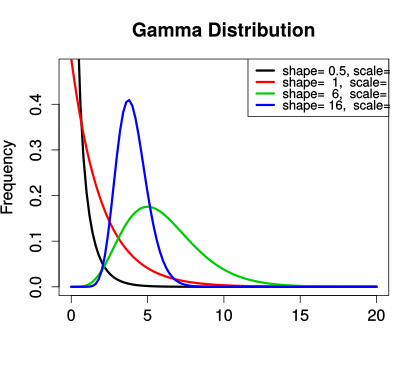
\includegraphics[width=7cm]{./Images/Gamma_dist.jpeg}
  \centering
  \caption{Example of different Distribution of Fitness Effects (DFE) represented by a gamma distribution.
  Many distributions can be represented by modifying the shape parameter of a gamma distribution, from
  a leptokurtic (shape parameter less than 1) to an exponential (shape parameter equal to 1) or a
  skewed normal distribution (shape  greater than 1).
   }
  \label{fig:Gamma}
\end{figure}


The divergence at the neutral sites is then proportional to the mutation rate per site and the predicted divergence at the selected sites, in the absence of advantageous mutations, 
is proportional to the product of the mutation rate and the average fixation probability of a selected mutation, 
which is inferred based on the DFE and other parameters estimated from the polymorphism data analysis
	\citep{Eyre-Walker2009}.
The difference between the observed and predicted divergences therefore estimates the divergence due to adaptive substitutions.

Using this method Eyre-Walker and collaborators 
In Drosophila genes, we estimate
that approximately 50\% of amino acid substitutions and approximately 20\% of substitutions in introns are adaptive
	\citep{Eyre-Walker2009}.

Molecular evolution simulations have been performed to test if the estimates of different tests, like the MKT and the more sophisticated DFE-alpha, are accurate under different realistic gene-structure and selection scenarios
	\citep{Messer2013}.
More specifically, the authors wanted to test how accurate these methods are in presence of genetic draft (stochastic effects generated by recurrent selective sweeps at closely linked sites)
and background selection (interference among linked sites by lightly deleterious polymorphisms).

They found that in the presence of slightly deleterious mutations, MKT estimates of $\alpha$ are severely underestimated.
They also found that the DFE-alpha is very accurate to calculate alpha when changes is demography are considered
	\citep{Messer2013}.
.




	\clearpage
	\section{Drosophila}
	


\subsection{Subsection one}


\subsubsection{Subsubsection one}


	\clearpage
	\section{Ciona}
	\subsection{Ciona as a model}
	The ascidian \textit{Ciona intestinalis}, a marine invertebrate animal, has a long history in developmental biology and evoutionary biology. 
	Darwin highlighted the importance of the ascidians due to their  close phylogenetic relationship to the vertebrates (REF). 
	Also, it provided one of the first evidences of localized determinants of cell specification \citep{Conklin1905}. 
	Although their adult form is a sessile filter feeder, its tadpole larva has characteristic features of the chordate group: a dorsal neural tube, a notochord surrounded by muscle and a ventral endodermal strand (Satoh, 1994).
	Ascidians show morphogenetic movements during gastrulation and neurulation similar to vertebrates and both share common genetic regulators of cell specification (REF).
	Their relative short life cycle, almost transparent body and rapid development facilitate many genetic techniques and are partly responsible for the re-emergence of \textit{C. intestinalis} as model organism in developmental biology \citep{Levin2012}.
	
\subsection{Current knowledge about Ciona development}
	The sequencing of the \textit{C. intestinalis} genome \citep{Dehal2002} facilitated its comparison with other vertebrate sequenced genomes and the analysis of gene expression through its life cycle.
	The \textit{C. intestinalis} genome is only 160Mb and contains ~16,000 genes, a gene number similar to the invertebrate \textit{D. melanogaster} genome and only is half of the genes found in some vertebrates (REF).
	This low number of genes (compared to vertebrates) can be explained by the finding that many gene families or subfamilies have only one representative in \textit{C. intestinalis} \citep{Dehal2002}.
	Relevant efforts have been made to describe the spatial expression patterns of individual genes (REF).
	The spatial expression patterns of  >1,000 cDNA clones have been described using whole-mount in situ hybridization techniques at different developmental stages \citep{Imai2004}.
	 Importantly, the developmental stages included cover a wide temporal range, e.g., blastula, gastrula and tapole stages (REF).
	 Taking advantage of the ascidian invariant cleavage pattern and well described lineage analysis \citep{Conklin1905,Nishida1987}, the spatial expression of many genes have been described at the single cell level up to the early gastrula stage (REF), making this an invaluable resource to investigate the spatio-temporal dynamics of gene expression.


	\clearpage
%%%% -----------------------------------------------------------------
%%%% -----------------------------------------------------------------

\chapter{Aims of the study}
\vspace{1cm}
In this work, I have analysed publicly accessible spatio-temporal gene expression data of two model organisms, \textit{Drosophila melanogaster} and \textit{Ciona intestinalis}, together with population genomics data of \textit{D. melanogaster}.
Using a statistical approach, I address these following questions, which have been selected for the great interest they have aroused in the scientific community since the early days of developmental and evolutionary biology:

\vspace{1cm}
%%%%%%%%%%%%%%%%%%%%%%%%%%%%%%%%%%%%%%%%%%%%%%%%%%%%%%%%%%%%%%%%%%%%%%%%%%
\begin{enumerate}[label=\Roman*]

\item How do complexity and compartmentalization increase in the embryo during development?
\vspace{0.5cm}

\item Are there differences in the pattern of compartmentalization and complexity increase when comparing different species (i.e., \textit{D. melanogaster} and \textit{C. intestinalis})?
\vspace{0.5cm}

\item Can adaptation be found in specific anatomical parts of the embryo or developmental stages? 
\vspace{0.5cm}

\item Is the Hourglass model supported by evidence of natural selection when considering inter and intra-specific variation at the DNA sequence level?

\end{enumerate}
%%%%%%%%%%%%%%%%%%%%%%%%%%%%%%%%%%%%%%%%%%%%%%%%%%%%%%%%%%%%%%%%%%%%%%%%%%
\vspace{1cm}

%
%These questions have been selected for the great interest they have aroused in the scientific community since the early days of developmental and evolutionary biology.
%%
%The work presented here is based on and uses concepts from three main biology fields: 
%developmental biology, evolutionary biology and population genetics.
%Nowadays, the combination of these scientific fields constitute multiple research programmes. Modern evolutionary developmental biology (evo-devo) is the explicit combination of the first two fields.
%	\nomenclature{evo-devo}{Evolutionary developmental biology}


%%%% -----------------------------------------------------------------
%%%% -----------------------------------------------------------------

\chapter{Material and Methods}
\input{./Parts/Methods}

%%%% -----------------------------------------------------------------
%%%% -----------------------------------------------------------------

\chapter{Results and Discussion}
\input{./Parts/Results_Discussion}


%%%% -----------------------------------------------------------------
%%%% -----------------------------------------------------------------

\chapter{Concluding Remarks}

The study of organismal complexity during embryonic development presented here shows that there are commonalities and differences between \textit{D. melanogaster} and \textit{C. intestinalis}. Both species showed a non-linear increase in all complexity measures, while the most remarkable difference is the timing of the major change in complexity, which is earlier in \textit{D. melanogaster} (around gastrulation).
Another common pattern is the early increase in complexity when considering only transcription factors or growth factors (or other signalling molecules). This confirms the special role these genes have in early metazoan development. It could be therefore expected that the evidence presented here, regarding these type of genes, should be observed also in other species. 

One important result of this work is that within each species, the three complexity measures showed a similar pattern (even when it would not be necessarily the case; see section X). This means that altogether, these measures (compartmentalization, disparity and roughness) are reflecting a global pattern of increase in complexity in each species. Therefore, it could be hypothesized that a similar increase in complexity would be found using alternative measures of complexity (e.g., spatial entropy). Further analysis would be required to test this hypothesis.
Also, the Synexpression Territories analysis allowed to "reconstruct" the main embryonic differentiation events in both species in a consistent manner with the current knowledge of the development of these model organisms and without focusing in specific genes.

The elaboration of an adaptation map on the fruit fly embryo can be considered a proof of concept of how the combination of diverse fields like evolutionary developmental biology and population genomics, and new techniques such as the phylostratigraphy, can be useful to give a fresh view on an old problem.
Using these maps, it was possible to visually identify that the center (internal part) of the embryo expresses a more conserved and older transcriptome, while the outside (external part) expresses phylogeneticaly younger and less conserved genes. This evidence seems to support the hypothesis of the antecedence of the endoderm with respect to the ectoderm \citep{Hashimshony2014}. It would be interesting to extend this adaptation mapping analysis for the entire development (until the adult stage) as it could be that in later stages, different structures or organs have been under positive or negative selection.

The estimation of adaptation over the entire life cycle of \textit{D. melanogaster}, as presented here, supports the HG model of development. We find, as other analyses previously have, that the mid-embryogenesis is highly conserved. The work presented here is different from previous ones in that it uses a more complete spatio-temporal dataset and a method that uses inter and intra-specific DNA coding variation to estimate, with an unprecedented precision, the proportion of adaptive changes.

Furthermore, as a result of this work is hypothesized that the hourglass model can be partially explained by various genomic features. However, further work is necessary to test this hypothesis.

%In here, I have taken advantage of the great amount of information about developmental gene expression that has accumulated in many years from collective efforts of the developmental biology community. This great amount of accumulated data allows to shift the focus from single genes to a systemic approach in which the global statistical properties of development can be investigated.


OPEN QUESTIONS AND FUTURE DIRECTIONS

The emergence of new techniques, like "spatial transcriptomics" of tissue sections at single-cell resolution \citep{Stahl2016} could make possible to have information, derived from a single experiment, of all the genes expressed in a 2D section of an embryo. The application of the measures presented here could be apply to this kind of data in a straightforward manner, solving the limitation in resolution of the work presented here.

It is important to mention that this work has used differential gene expression in the embryo and its spatial distribution as a tool to investigate complexity. However, embryonic development can not be reduced to differential gene expression. Cellular behaviours and the physical properties of the cells and tissues have also a causal role in the developmental process. It would be interesting to be able to measure the differential apportionment to complexity increase of the different developmental mechanisms.


The increase of organismal complexity and the study of adaptation during development remain fascinating topics after many centuries, and still offer many open questions to be solved. The incredibly fast pace of data generation, the development of new techniques and sophisticated methods give hope to finally open the black box of development.

%%%%%% for results of compartmentalization
%
%It could be expected that these early increase in complexity in drosophila is shared by all insects with a syncitial blastoderm stage. It could be that there are differences between these based on the number of cell divisions until the blastoderm is cellularized. It is known that Drosophila cellularizes relatively late (so there is more time for patterning within the syncitial bastoderm). In contrast, the desert locust (Schistocerca gregaria) cellularization occurs very early, before the formation of the blastoderm (REF Ho).
%
%The rapid development in drosophila could be due to selective pressures on the time of development, caused by the the eggs being layed ephemeral resources such as decaying fruits (this classical view has been chalenged recently; reviewed in REF Prasad). 
%The embryonic development of D. melanogaster takes around 1 day at 22 degrees. Even when developmental time can vary in a three fold manner depending on the Drosophila species and temperature (D. virilis embryonic development at 18 C takes more than 45 hours, compared to less tha 15 hours at 30 C in D. ananassae: REF Kuntz), it can be considered fast compared the dessert locust. In the locust, embryonic development takes around two weeks in calid environments in West Africa but it can take up to 70 days in the cooler temperatures of North Africa (REF locushanbbook).
%
%Also, it would be interesting to know if there are some differences between the two main modes of segmentation in insects, i.e., short germband and long germband. The red bettle (Tribolium castaneum) is most popular short germband inset that serves as a developmental biology model organism. Many valuable resources have become available in the last decades/years (REF Bucher). 
%
%
%The period of egg development, between laying and hatching, is called the incubation period. The rate at which eggs develop varies according to the soil temperature. For example, in the summer breeding areas of West Africa, the Red Sea coast and lowland India the incubation period takes 10-14 days but this is extended to 25-30 days in the cooler spring breeding areas of central Arabia, southern Iran and Pakistan while in North Africa it can take as long as 70 days in exceptionally cold weather


%%%% -----------------------------------------------------------------
%%%% -----------------------------------------------------------------

\listoffigures
%\printnomenclature
%%%% -----------------------------------------------------------------
%%%% -----------------------------------------------------------------

%\bibliographystyle{plain}
\bibliography{Bibliography}

%%%% -----------------------------------------------------------------
%%%% -----------------------------------------------------------------
\end{document}